\section{Creating the Index}

The first task was to create a Lucene Index on the Cranfield Documents. The main() method parses the command-line parameters, then in preparation for instantiating IndexWriter, opens a Directory, and instantiates StandardAnalyzer and IndexWriterConfig. The Cranfiled Documents to be indexed is imported from the command line providing the location of the document. The value INDEX\_DIRECTORY is the path in which the filesystem directory where all index information should be stored.  \par 

Inorder to index and process all the docuemtns I created a parser for the Cranfield file .The Cranfield file was a list of documents where each document had a Title (I.), Author (A.), Bibliography (B.) and the text (W.). The parser would read the file in line by line. Each line would be added to an variable depending on the filed. Once the parser looped abck to a title context the variables would create a new document. \par 
	
Upon completion of all the documents being created, they were added to an ``IndexWriter" object and also written to a Directory. This directory was analysed applying a  a modified Analyzer which I created. \par

This analyser normalised characters to lower case, removed stop words and stemmed the words. Removing the stop words were words taken from the ENGLISH\_STOP\_WORDS\_SET in the ``StopAnalyser" libray. The ``PorterStemFilter" library was used to stem the words when being indexed.   \newline

	\begin{figure}[ht!]
		\begin{center}
			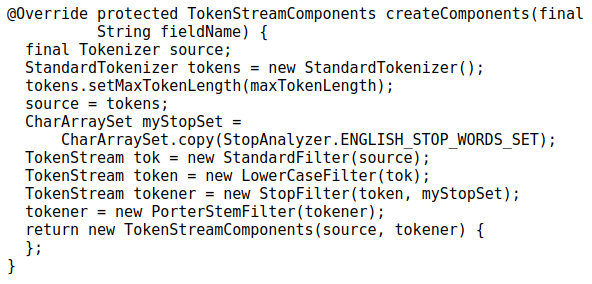
\includegraphics[scale=.325 ]{2} 
			\caption{Code Snippet of the anlayser used to stem and remove stop words}
			\label{fig:1}
		\end{center}
	\end{figure} \par

\newpage
\section{Querying the Index}
Once I created the Index I had to begin to search the index. With the multiple fields the index contained for each document I used a ``MultiFieldParser" which searched the document for each field. The only issue was that it treats each field equally when searching in the documents.  I decided to alter weighting of importance for each field. \par

	\begin{figure}[ht!]
		\begin{center}
			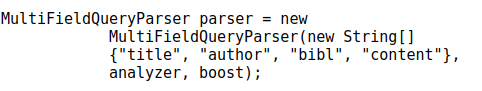
\includegraphics[scale=.5 ]{6} 
			\caption{Code Snippet of MultiFieldParser}
			\label{fig:1}
		\end{center}
	\end{figure} \par
  
In order to determine the weighting for each field, a number of tests were done to find the most accurate weightings to give the best results. From previous experience of searching for books, I would never use the Author or Bilbiography to search for a speicfic book so I gave them a lower weighting of importance. The title and context were the main fields so they had a much higher weighting. \par

	\begin{table}[H]
		\centering
		\begin{tabular}{|p{2.5cm}|p{2.5cm}|}
			\hline
			\textbf{Context} 	& \textbf{Weighting} \\ \hline
			Title 				& .45 \\ \hline\hline
			Author 				& .11 \\ \hline\hline
			Bibliography 		& .02 \\ \hline\hline
			Content 			& .41 \\ \hline\hline
		\end{tabular}
		\caption{Weight of each field}
		\label{table:weight}
	\end{table}

The queries were parsed from the ``cran.qry" file. They were then, just like the index file were then stemmed and removed stop words using the customised Analyser. Once all the queries were in the same format as the index file they were then put into the ``IndexSearcher" which searched the index for each query and returned all the matching documents. I set the amount of documents to be returned to be 30 results to only return the highest results.    

	\begin{figure}[ht!]
		\begin{center}
			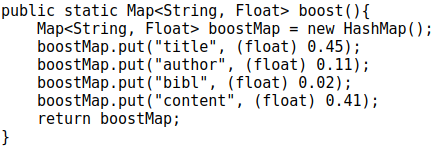
\includegraphics[scale=.4]{4} 
			\caption{Code Snippet of weighting the fields}
			\label{fig:1}
		\end{center}
	\end{figure} \par

\newpage
\section{Scoring}

The ``IndexWriterConfig" has a method called ``setSimilarity" which sets the type of Lucene scoring that you would like to use. Similarity defines the components of Lucene scoring. From research the main four lucene scoring methods are: \par
		
	\begin{multicols}{2}
		\begin{itemize}
			\item BM25
			\item Boolean
			\item Classic
			\item lm\_dirichlet
		\end{itemize}
	\end{multicols}
	
One of the higher-level implementation such as TFIDFSimilarity (also known as Classic Similarity), which implements the vector space model with this API is one of the four I decided to use. \par 

	\begin{figure}[ht!]
		\begin{center}
			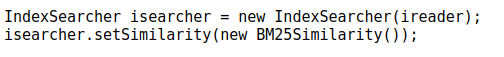
\includegraphics[scale=.5 ]{5} 
			\caption{Code Snippet of setting the Similarity when Searching}
			\label{fig:1}
		\end{center}
	\end{figure} \par

When testing it was necessary to make sure that the indexing and query searching were using the same similatiry scoring as they had to be the same in order to get the right results and scores. \par
 
	\begin{figure}[ht!]
		\begin{center}
			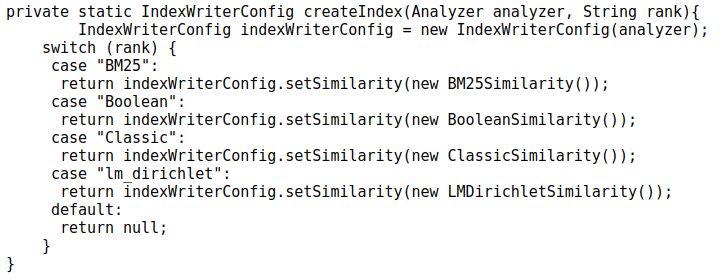
\includegraphics[scale=.35 ]{3} 
			\caption{Code Snippet of diffferent Scoring Similarities when Indexing}
			\label{fig:1}
		\end{center}
	\end{figure} \par

\section{Results}

	\begin{table}[H]
		\centering
		\begin{tabular}{|p{2.5cm}|p{2.5cm}|}
			\hline
			\textbf{Similarity} 	& \textbf{Score} \\ \hline
			BM25 				& .45 \\ \hline\hline
			Boolean 				& .11 \\ \hline\hline
			Classic 		& .02 \\ \hline\hline
			lm\_dirichlet 			& .41 \\ \hline\hline
		\end{tabular}
		\caption{Results of each scoring method}
		\label{table:weight}
	\end{table}
	
\newpage
\section{Conclusion}
